% Chapter 10

\chapter[Testing]{Testing} % Main chapter title

\label{Chapter10} % For referencing the chapter elsewhere, use \ref{Chapter10} 

%----------------------------------------------------------------------------------------

Software testing is the practice of defining a number of processes which can be applied to a piece of software in order to verify its correct operation. Each of these processes may involve a number of steps, and is usually described as a single test. The results of each test are normally compared against some expected, correct outcome, and used to determine if any bugs or issues remain in the software. It was important to thoroughly test the software in order to verify its correct implementation and operation, and identify any remaining issues that needed to be fixed or mitigated. Some testing was done throughout the implementation phase, after each feature addition, and this testing is referred to here as continuous integration testing. More rigorous testing processes were then applied once the implementation was complete, including testing of both the user interface and the system back end, as well as testing the system as a whole. This section gives details of the different testing processes applied to the system, the results obtained, and details of any resulting fixes that were implemented.

%----------------------------------------------------------------------------------------

\section{Continuous Integration Testing} \label{ContinuousIntegrationTesting}
The purpose of the continuous integration testing was to verify the correct operation of individual components as they were completed, and to ensure that different components would work correctly together. This was done during development to reduce the risk of issues stacking up and becoming layered or entrenched as development continued. The modular design of the software made the continuous integration testing process relatively simple. After a software component or a specific functionality was implemented, it was tested informally by supplying relevant data or control inputs and verifying the correct result. The existing modules and functionality were then also re-tested. This helped to check that the newly implemented functionality had not created an issue elsewhere. Where possible each module was also tested in isolation, prior to being connected to any related modules, to avoid issues becoming compounded. For example the \textit{MachineVision} class was tested alone, by verifying that it could retrieve a single image from the camera and track the robots in said image, before it was connected to the higher level \textit{CameraController} component. Another example was the testing of the networking code in isolation, which involved using an external tool to supply individual UDP packets, and verifying that they were correctly received by the \textit{DataThread} class by outputting their raw contents. 

The continuous integration testing was completed in a relatively informal manner, as the main focus at the time was implementation, however it was still a useful technique and helped to ensure that bugs were caught early when possible. For a larger, more complex application, being developed by a team rather than an individual, integration testing should be applied in a more formal manner. For this application however it was deemed more important to focus on the actual implementation, due the relatively limited time available.

%----------------------------------------------------------------------------------------

\section{Manual User Interface Testing} \label{ManualUserInterfaceTesting}
The purpose of any graphical user interface is to present information to a human user and collect their input. It is therefore important that user interfaces be tested manually by a human user, as automated testing methods are often not sufficient for, or not capable of, verifying that information is displayed legibly and correctly, and that user input functions properly. The user interface of the system is one of the most important parts of the project, and therefore a thorough manual user interface testing process was undertaken.

\subsection{Method}
The general approach taken to the user interface testing can be summarised as follows:

\begin{enumerate}
 \item Separate UI into individual elements.
 \item State the purpose and required functionality of each element.
 \item Define a general test strategy for an arbitrary single UI element as a series of checks.
 \item Identify any special case components, and define different test strategies where necessary.
 \item Apply the relevant strategy to each interface element in turn.
\end{enumerate}

\vspace{0.5cm}

\noindent The user interface was separated into the elements described in table \ref{tab:UserInterfaceElements}. Special case elements requiring different test strategies are highlighted in bold.

\begin{longtable}{ l c }
 Element & Test Strategy\\
 \hline
 Visualiser Panel Tab System & A \\
 \textbf{Visualiser} & \textbf{B} \\
 Visualiser Settings Tab & A \\
 Camera Settings Tab & A \\
 Robot List Panel Tab System & A \\
 Robot List Element & A \\
 Network Settings Tab & A \\
 Logging Settings Tab & A \\
 Data Panel Tab System & A \\
 Console Data Tab & A \\
 Overview Data Tab & A \\
 State Data Tab & A \\
 IR Data Tab & A \\
 Custom Data Tab & A \\
 Individual Visulisation Settings Dialogs & A \\
 \bottomrule
 \caption[User Interface Elements for Testing]{Individual user interface elements that required testing, and the test strategy applied.}\\
 \label{tab:UserInterfaceElements}
\end{longtable}

\noindent The following test strategies were then devised for the different element categories.

\textbf{Test Strategy A - Standard UI Elements:}

\begin{enumerate}
 \item Examine UI element visually. Verify that it appears correct. Verify that it contains all elements necessary to satisfy its purpose.
 \item Examine all text within the element. Check for errors in both meaning and spelling.
 \item Verify that all components within the element which perform actions in response to user input operate correctly.
 \item Verify that all components respond quickly to user input.
 \item Verify that component actions and functionality do not degrade with extreme use (sustained rapid input, large numbers of input changes, extreme or out of range values, etc).
 \item Verify that all data displayed within the element is visible, readable, correctly arranged and correctly labelled.
 \item Verify that the element behaves sensibly when window resizing occurs, and that it remains usable and data remains visible whenever possible.
 \item Verify that the element updates promptly when responding to changes in data.
\end{enumerate}

\textbf{Test Strategy B - Visualiser:}

\begin{enumerate}
 \item Verify that the video image is displayed correctly.
 \item Verify that user clicks within the visualiser space are located correctly, at a number of different window sizes.
 \item Verify that robots can be selected by clicking on their location in the visualiser image.
 \item For each data visualisation type:
 \begin{enumerate}
  \item Define a set of input data and the expected representation of this data.
  \item Supply the input data.
  \item Verify the representation is as expected.
  \item Check that the visualisation is clear and any text is legible.
  \item Repeat for multiple sets of input data.
  \item Verify that integrity is maintained with extreme data, corner cases and zero data, wherever possible.
  \item Verify that integrity is maintained at a range of window sizes, within reasonable limits.
 \end{enumerate}
\end{enumerate}

\subsection{Results}
For each user interface element the appropriate test strategy, as specified in table \ref{tab:UserInterfaceElements}, was carried out. The results of this testing can be found in appendix \ref{app:UITestResults}. The testing highlighted no major problems with functionality, but did identify a number of smaller issues, mostly related to aesthetics and usability.

\subsection{Fixes Implemented}
The following fixes were implemented to address the issues identified during the manual user interface testing:

\begin{itemize}
 \item The settings tabs in the visualiser panel were renamed to better reflect their purpose.
 \item Long directory paths in the logging tab were truncated to only display the final 25 characters.
 \item The ordering of messages in the console was reversed, to read from top to bottom in the order that they occurred.
 \item The redundant heading was removed from the overview tab.
 \item Entries in the state transition list were reformatted to clearly separate the time-stamp from the states.
 \item The IR data tab was reorganised to be more space efficient, and display data more clearly. Headings and labels were added to further improve clarity.
 \item Code was added to flip the video image, and a setting was added to the camera settings tab to enable and disable this feature.
 \item Robot IDs rendered in the visualiser were positioned slightly closer to the robot's horizontal position.
 \item The IR data visualisation in proximity mode was adjusted to have a shorter maximum line length, and to use a non-linear mapping to improve the proximity approximation.
 \item The IR data visualisation in heat mode was adjusted to use white as the base colour for clarity, changing to red and increasing in size with increasing sensor value.
 \item An upper limit was added to the robot path sampling interval.
\end{itemize}

%----------------------------------------------------------------------------------------

\section{Data Model and Back End Unit Testing} \label{BackEndUnitTesting}
The next large code component requiring testing was the data model, which formed the majority of the application back-end code. Testing the data model manually, by inputting data packets and verifying the correct insertion of data into the model, was deemed to be too time consuming. This manual approach also posed another problem, in that the contents of the data model could only be examined through the user interface, which meant that the data model testing would be inherently coupled to the UI. This would make it harder to determine the source of any bugs found, as they might be related to the data model or the UI. Avoiding this kind of interdependency is part of the reason for adopting an object oriented approach to the software design and implementation. In order to avoid this issue, the back-end was tested using an automated, 'unit-testing' based approach.

Unit testing is a commonly used technique in professional software testing \cite{UnitTesting}, and involves writing specific functions or scripts which test individual 'units' of code in an automated fashion. These test cases will manipulate the unit in some way, using the data and functions it exposes. Then the test case will assert a fact that should be true after the manipulation, such as a comparison of a data point within the unit and the value it should have following the given operations. Each test might include many of these assertion statements, and the test only passes provided that all assertions evaluate to be true. In order to apply this technique to this system, an extra class - `\textit{TestingWindow, testingwindow.cpp / .h}' - was added to the application. Alongside this class a number of individual test case functions were added. Each of these functions was written to test the data model in a specific way. Table \ref{tab:DataModelTestCases} lists the test case functions and their purposes.

\begin{longtable}{ l p{10cm} }
 \textbf{Test Case} & \textbf{Purpose and Method}\\
 \hline
 Robot Insertion Test & Tests whether data objects for new robots are inserted into the model correctly. Supplies a packet of each possible type, using a new robot ID each time. Asserts after each packet that the number of robots stored in the model has increased by one. Supplies another set of packets, this time reusing the existing robot IDs. Asserts after each packet that the number of robots stored in the model has not increased.\\
\hline
 Name Data Test & Tests whether data describing the name of a robot, received in watchdog packets, is inserted into the data model correctly. Supplies three watchdog packets, each with a different robot ID and robot name. Asserts that the data model now contains three robots, and that their name data matches the names entered in the packets. Supplies three new watchdog packets for the same set of robot IDs, with different names. Asserts that the data for each of the robots has been updated to include the new name data.\\
\hline
 State Data Test & Tests whether data describing the current state of a robot, received through state packets, is inserted into the data model correctly. Supplies three state packets, each with a different robot ID and state. Asserts that the data model now contains three robots, and that their state data matches the states entered via the packets. Supplies three new state packets for the same set of robot IDs, with different states. Asserts that the state data for each of the robots in the model now matches the new states.\\
\hline
 Position Data Test & Tests whether packets describing the current position and orientation of a robot are correctly parsed and the data stored correctly in the data model. Supplies three position packets, each with a different robot ID and different position values. Asserts that the data model now contains data for three robots. Asserts that this data matches the values in the packets for x-position, y-position and angle individually. Supplies three more position packets for the same set of robot IDs with new position and angle values. Asserts that the data in the model for each robot has been updated to reflect the new values. Assertions involving floating point numbers are done using a tolerance comparison, with a tolerance of $ 1 \times 10^{-7} $.\\
\hline
 IR Data Test & Tests whether packets describing a robot's infra-red sensor values are correctly parsed and the data correctly stored in the data model. Supplies an IR data packet, with each sensor reading containing a different value. Asserts that the IR data in the model matches each of the values in turn. Supplies another IR data packet with new, unique values. Asserts that the IR data in the model now matches each of the new values. This process is repeated for packets of background IR data type.\\
\hline
 Custom Data Test & Tests whether packets describing custom data key/value pairs are correctly parsed and the data correctly stored in the data mode. Supplies three custom data packets, each with a different robot ID and a different value, for a single key. Asserts that the data model now contains data for three robots, and that each robot has a custom data entry for the given key. Asserts that the value for each of these entries matches the value supplied in the relevant packet. Supplies three new packets for the same set of robots with a new key and a new value. Asserts that each robot now contains custom data for the second key, and that the values match those supplied in the packets. Supplies three more packets using the original key, with new values. Asserts that the values for the original key for each robot have been updated to match the values in the latest packet set.\\
\hline
 Position History Test & Tests whether position data supplied for a robot is correctly sampled and stored in the position history portion of the data model. Sets the position history sampling rate to 2. Supplies twenty position packets, all attributed to the same robot ID. Asserts that the position history now contains ten entries. Asserts that the x- and y-position values for each of these entries match the values in every second packet, in reverse order. Assertions involving floating point numbers are done using a tolerance comparison, with a tolerance of $ 1 \times 10^{-7} $.\\
\hline
 State History Test & Tests whether the state transition history data is correctly formed from a sequence of state packets. Supplies five state packets, each attributed to the same robot ID and containing different states. Asserts that the state transition history now contains five entries. Asserts that the entries describe the correct state transitions, as described by the packets, in reverse order.\\
\hline
 Bad Data Test & Tests whether badly-formed data packets are correctly rejected by the data model. Supplies a number of correctly formed data packets, each with a different robot ID, and asserts that the data model now contains the correct number of robot entries. Supplies a number of invalid and malformed data packets, distributed between the already used robot IDs and several new IDs. Asserts that the number of robots in the model has not changed, and that the data in each of the existing robots has not changed.\\
 \bottomrule\\

 
\caption[Data Model Test Cases]{Test cases used to unit-test the data model.}\\
 \label{tab:DataModelTestCases}
\end{longtable}

The \textit{TestingWindow} class displays an additional user interface window, which can be opened by selecting the `\textit{Testing Window}' option from the developer menu on the main tool-bar of the application. This window displays a list of the available tests, a text area for displaying test results, and controls for running either a single test or the full set. Each time a test is run the class instantiates a new data model object, performs the operations for the test in question, displaying the steps involved as text in the results window. For each assertion the text describes what is being asserted and states whether the result was true or false. The overall result of each test is then stated at the end, and the data model object is destroyed. This therefore allows any developer working on the system to open this window at any time whilst the application is running and verify that the full set of tests still passes. This can be done whenever changes are made to the back end code, and gives the developer a degree of certainty that the data model is still functioning correctly. New tests can be easily added by implementing a new test function and adding it as a test case. The interface for this test window is shown in figure \ref{fig:TestingWindow}.

\begin{figure}
 \centering
 \makebox[\textwidth][c]{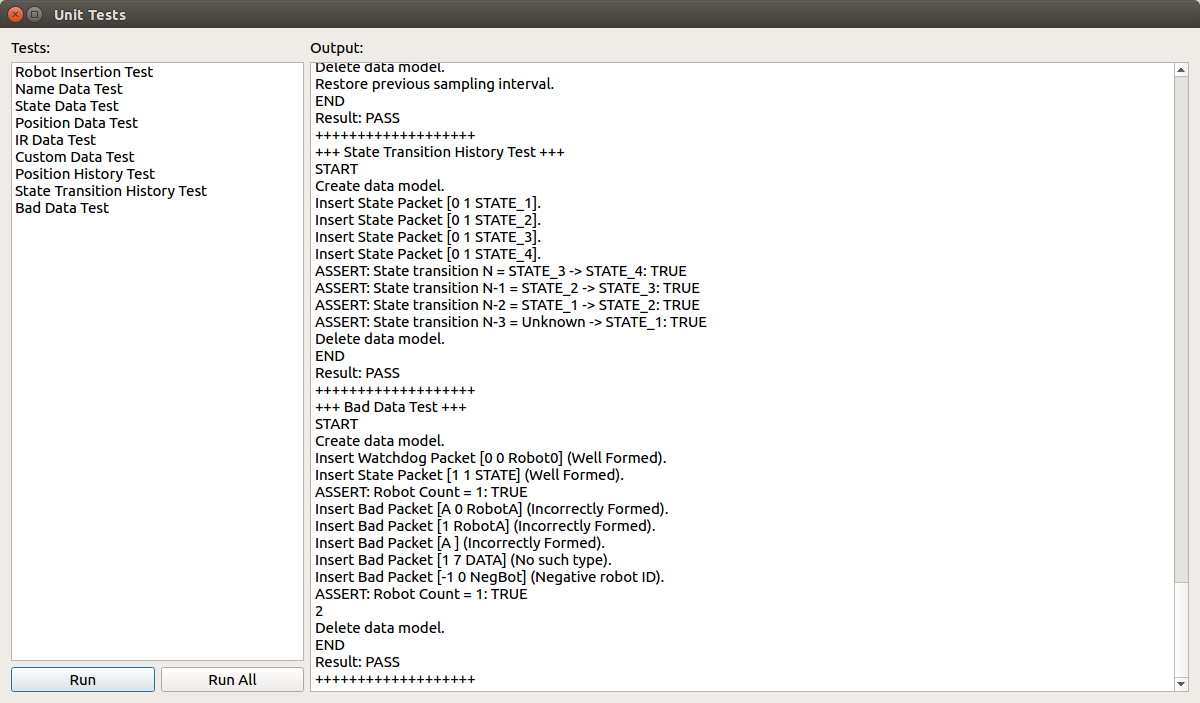
\includegraphics[width=1.2\textwidth]{Figures/TestingWindow.png}}
 \decoRule
 \caption[Testing Window]{The testing window, used for running the data model unit tests.}
 \label{fig:TestingWindow}
\end{figure}

\subsection{Results}
In its final state following this project the data model was implemented such that all of the stated test cases passed successfully when run. This indicated that the data model was implemented to a satisfactory standard, and that if data was supplied in correctly formatted packets, it would be correctly stored in the model. Other application functionality that relied on the data model could therefore be used and tested with the assumption that the model was operating correctly.

\subsection{Issues with this Approach}
The unit testing approach suffers from a number of issues. First and foremost the results of the tests are only as good as the tests themselves - meaning that any bugs in the code of each test could be misinterpreted as bugs in the software itself. To mitigate this the tests are designed to be as logically simple as possible, and perform the smallest number of operations necessary to achieve the behaviour under test. This minimises the chances of a mistake in the implementation of the test code. 

This approach also relies on the developer writing the tests correctly determining, and correctly entering, the required result for each assertion statement. One example of this issue is in floating point comparison. The accuracy with which a floating point variable can describe a number is inherently limited due to the way a floating point variable is constructed. In almost all cases a floating point number will differ from the exact value it is attempting to represent by some small amount. This can present an issue when performing comparisons between the contents of a floating point variable and an exact value, leading to false negatives. In order to avoid this all floating point comparisons have been done using a threshold, rather than a direct comparison. This technique asserts that when the expected value is subtracted from the variable being tested, the modulus of the result is less than some very small tolerance value, indicating that the value in the variable is within an acceptable range of the expected value. A tolerance value of $ 1 \times 10^{-7} $ was used in all test cases, as this was deemed to indicate sufficient accuracy for the data in this system. To give some perspective to this number, note that the x-position value of a robot is stored as a floating point value between 0 and 1, representing a portion of a physical distance of approximately two and a half meters. A discrepancy of +/- $  1 \times 10^{-7} $ therefore equates to an error of $ 0.25 mm $. Hence this tolerance value indicates more than adequate accuracy.

%----------------------------------------------------------------------------------------

\section{Verification and Validation Testing} \label{ValidationTesting}
Verification and validation (V\&V) testing \cite{VerificationTesting} is the process of determining whether the software implemented meets the high level requirements, and whether the individual functionalities operate correctly and without bugs. This was the last step in the testing process, and served to test the system as a whole. The approach taken was to consider the requirements of the system, as stated in the functional specification in section \ref{FunctionalSpecification}, and determine whether each requirement is satisfied by the functionality implemented. Where possible each functionality will be tested with relevant data and control inputs. The requirements, and the tests carried out for each are given below.

\noindent\textbf{Core Requirements}

\begin{enumerate}[label=C\arabic*.]
 \item Must comprise a PC application.
 \begin{itemize}
  \item Verify the software runs on a PC and/or server.
  \item Verify that the software has the general appearance of a software application.
 \end{itemize}
 
 \item Must be capable of receiving data related to the state of multiple robots.
 \begin{itemize}
  \item Program a number of robots to send state data through the system, and verify that it is received and displayed by the application.
 \end{itemize}
 
 \item Must be capable of receiving positional data for the same set of robots.
 \begin{itemize}
  \item Program the robots to move along a number of different paths in view of the system, and verify that their positioned are correctly tracked and displayed by the application.
 \end{itemize}
 
 \item Must be capable of receiving a live video feed of the robots in their environment.
 \begin{itemize}
  \item Run the application and verify that the video feed is displayed.
  \item Introduce a number of robots and objects to the environment space and verify that they are seen in the video feed.
 \end{itemize}
 
 \item Must collate received data and present it to the user in a combined graphical form.
 \begin{itemize}
  \item Program the robots to report a number of different data types, including sensor data, and verify that this can all be displayed by the application simultaneously.
 \end{itemize}
 
 \item Must present auxiliary, non-spatial data to the user in textual or other forms.
 \begin{itemize}
  \item Program the robots to report name, state and custom data and verify that this is correctly received and displayed in the application.
 \end{itemize}
 
 \item Must update in approximately real time.
 \begin{itemize}
  \item Program the robots to report data periodically, and verify that the data within the application updates in real time.
  \item Program the robots to move around in view of the system, and verify that the video shows their movement in approximately real time.
 \end{itemize}
 
 \item Must at minimum support the e-puck robot platform.
 \begin{itemize}
  \item The previously stated tests should be performed using e-puck robots.
 \end{itemize}
\end{enumerate}

\textbf{Secondary Requirements}

\begin{enumerate}[label=S\arabic*.]
 \item Should use a modularised structure.
 \begin{itemize}
  \item Verifying this through standard testing is not feasible. See section \ref{ApplicationStructure} for details of the modular implementation.
 \end{itemize}
 
 \item Should exchange data between the robot platform and the application using a platform-agnostic, extensible protocol.
 \begin{itemize}
  \item Use a platform other than the e-puck robot to transmit packets to the application. Verify that the packets are received and interpreted correctly regardless of the source.
 \end{itemize}
 
 \item Should provide a basis for interoperability with a number of robotics platforms.
 \begin{itemize}
  \item Verifying this requires another robot platform to be integrated into the system. This is outside the scope of the project. However sections \ref{DataTransferFormat} and \ref{RobotSide} indicate how the system has been implemented with portability in mind, and suggest that interoperability should be feasible and relatively easy to achieve.
 \end{itemize}
 
 \item Should allow the user to configure the displayed data.
 \begin{itemize}
  \item Program the robots to report data of all supported types. Verify that the visualiser settings allow for display configuration.
 \end{itemize}
 
 \item Should employ a model-view-controller (MVC) software architecture.
 \begin{itemize}
  \item Verifying this through standard testing is not feasible. See section \ref{SoftwareArchitectureDesign} for details of the MVC based architecture design.
 \end{itemize}
 
 \item Could provide the user with ways to configure and display custom data types.
 \begin{itemize}
  \item Program the robots to report a variety of textual and numerical custom data. Verify that this data is received, stored and displayed correctly.
  \item Verify that the custom data overlay can correctly display any of the received data.
 \end{itemize}
 
 \item Could allow the user to compare data on two or more specific individual robots.
 \begin{itemize}
  \item Due to time constraints, and a lack of interest in this feature during the initial survey, it was deemed low priority, and ultimately not implemented.
 \end{itemize}
 
 \item Could calculate and display swarm-level meta-data and statistics.
 \begin{itemize}
  \item Verify that the average position of the tracked robots is correctly displayed.
 \end{itemize}
 
 \item Could generate log files of robot activity over a user defined period.
 \begin{itemize}
  \item Program the robots to periodically report data of various types. Verify that pressing the start logging button, and then pressing it again (to stop the logging) some time later, results in the generation of a log text file containing entries for all data received in the time period between the presses.
  \item Verify that setting the log file path directory using the user interface correctly affects where the log file is saved.
 \end{itemize}
\end{enumerate}

\subsection{Results}
\begin{longtable}{ l p{10cm} }
 \textbf{Test} & \textbf{Result}\\
 \hline
 C1 & The application was run successfully on two machines running Linux operating systems. The application has an appearance consistent with the familiarly understood definition of a software application.\\\hline
 C2 & Data of all defined types was successfully sent from six robots to the application. The data was correctly displayed within the application.\\\hline
 C3 & The positions of six moving robots were correctly tracked simultaneously. The tracking data obtained was correctly displayed in the application both numerically and visually.\\\hline
 C4 & The application correctly displays the input video feed. Objects placed in view of the camera are seen in the video feed within the application.\\\hline
 C5 & Data received from the robots, including sensor data, was correctly converted to visual representations and displayed in the application.\\\hline
 C6 & Data received from the robots was correctly received and displayed in a textual form within the application.\\\hline
 C7 & The application updated the data displayed to match new data from the robots in approximately real time. The application updated the position and orientation data to match the movement of the robots in approximately real time.\\\hline
 C8 & E-puck robots used for all core tests involving robots. The e-puck platform is sufficiently supported.\\\hline
 \hline
 S2 & Utility program used to send specific UDP packets to the application via the network, mimicking the behaviour of an arbitrary robot. The system received and interpreted the packets correctly.\\\hline
 S4 & The visualisations of the data reported by six robots could be configured using the options available in the visualiser settings menu, to a moderate extent. Full customisation of all aspects of the visualisations was not possible.\\ \hline
 S6 & Custom data sent from six robots was received and displayed within a table correctly, updating in approximately real time. The custom data visualisation could be set to target any of the specific data points received. The target data point was then correctly displayed, overlaid on the video feed. Configuring the display of custom data beyond a textual representation was not possible. Displaying more than one target data point was not possible.\\\hline
 S8 & When enabled, the average position display correctly displayed the average position of the currently tracked robots as a mark within the video feed, when tested with three, four and six robots. This data was not provided in numerical form. Other swarm-level data was not provided.\\\hline
 S9 & Was able to correctly start and stop logging whilst receiving data from six robots. The generated text file contained appropriate information. The layout of this information was, however, difficult to parse, making the data hard to understand and use. The directory to store the log files could be correctly set using the UI controls.\\\hline
 \bottomrule\\
 
 \caption[Verification Testing Results]{Verification testing results.}\\
 \label{tab:VerificationTestResults}
\end{longtable}

\subsection{Analysis}
All core requirement tests, C1 through C8, passed satisfactorily, indicating that the application satisfies the core requirements. Secondary requirement test S2 passed satisfactorily, without caveats. Verifying secondary requirements S1, S3 and S5 was not possible using standard testing approaches. Secondary requirement S7 was dropped following the results of the initial user survey, and a reassessment of the feature set. Tests S4, S6, S8 and S9 all passed conditionally, as the requirement was either partially met, or met to a limited standard. In order to fully satisfy these secondary requirements the following developments could be made in the future:

\begin{itemize}
 \item S4: Further develop the visualisation configuration options to allow the user to fully configure all visualisations, including sizes, offset positioning, font sizes, line widths, etc.
 \item S6: Develop the visualisation of custom data to allow the user a number of graphical options. Allow the user to visualise more than one custom data point simultaneously.
 \item S8: Add a new tab to the data panel for swarm-level data acquired through analysis. Display the average position values in this tab. Define and implement a number of other swarm-level data analyses, and display this data within the tab, as well as graphically within the visualiser.
 \item S9: Edit the log file generation to produce more structured files, using a comma-separated-value (CSV) format or similar.
\end{itemize}


%----------------------------------------------------------------------------------------

\section{Summary}

This chapter has described the methods used to test the application software and verify its correct operation. The process of manual user interface testing was discussed, and the test strategies for this application defined. The results of these tests were presented and the resulting fixes described. The use of unit-test style code build into the application for testing the data model was also discussed. The results of the verification and validation testing were used to verify that the software satisfied the functional specification defined in section \ref{FunctionalSpecification}. Overall these tests confirmed that the application functions correctly, and only minor fixes were required.